\chapter{\leavevmode\newline Introduction}
\label{chap:Introduction}

Advanced driver assistance systems (ADAS) have gained significant attention as a revolutionary technology for improving travel experiences, aiming to enhance safety, providing active assistance to drivers, and facilitating the development of fully autonomous driving technology. To handle the complex road geometry and topology, multi-agent interactions, and accurately follow the high-level command such as routing information, the machine learning algorithms have been widely integrated for ADAS and are becoming popular in this decades \parencite{chen2019model} \parencite{shaout2022adas}.

\begin{figure}[h]
\centering
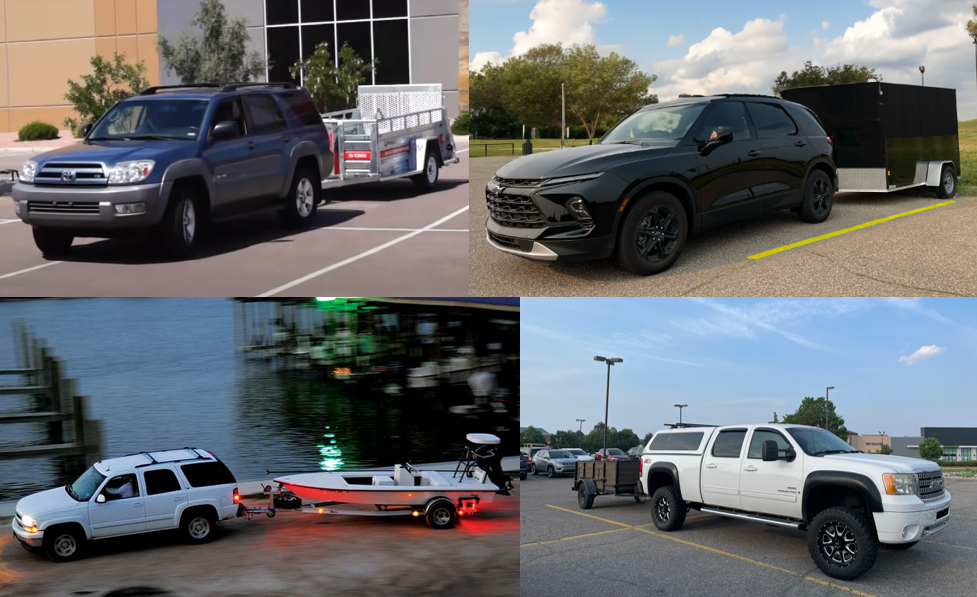
\includegraphics[scale=0.5]{fig/trailer_parking_real_world_all.png}
\caption{Truck trailer system in daily life}
\label{fig: real world trailer parking}
\end{figure}

Among the various features of ADAS, the control and auto-parking assist systems for tractor-trailer wheeled robots (TTWR) have gained significant attention in recent years, because of trailer vehicles' ability to significantly increase load capacity at a relatively low cost, resulting in more efficient use of resources and reduced transportation costs for achieving cooperative tasks\parencite{liu2022review}. However, the nonlinear, nonholonomic, unstable, and under-actuated system behaviors, along with the large blind zone behind the trailer make TTWR reverse parking a challenging and stressful experience. Another difficult part of the system is the phenomenon called jackknife, which occurs when the angle between the tractor and trailer is beyond a certain threshold, which prevents the driver from steering or aligning the trailer properly during driving backward. When the TTWR system is in the jackknife state, the steering maneuver has little effect on controlling the trailer's states.

Extensive research, for decades now, has been dedicated to addressing the challenges associated with TTWR systems, resulting in the development of various controlling methods that use controllers such as fuzzy logic, neural networks, and nonlinear controllers. For example, traditional control techniques, including Proportional-Integral-Derivative (PID) and model predictive controllers, have been widely utilized in Jackknife prevention, as well as other systems such as steer-by-knob. Jing et. al \parencite{jing2019control} solved the tractor-trailer reverse motion by designing three distinct controllers using a proportional integral controller, a sliding mode controller, and a neural network controller respectively. Moreover, a generic control safety governor was developed to supervises the tracking algorithms, overriding control to ensure jackknife-free operation. Xu et. al \parencite{xu2023improving} revisited Proximal Policy Optimization (PPO), enhancing it through two main innovations: firstly, they reformulate PPO into a linearly combined form to control the trade-off between accumulative discount return and divergence, addressing parameter tuning complexities, and secondly, they introduce a parametric alpha divergence in place of the traditional Kullback–Leibler (KL) divergence for more effective policy differentiation. The novel variant, alphaPPO, is validated across six benchmark environments, outperforming existing PPO forms. The work contributes a more effective balance in return and divergence, and a refined divergence measurement, broadening PPO's application in reinforcement learning. Zanchetta et. al \parencite{zanchetta2019trailer} propose a method to control the trailer's lateral position through vehicle yaw moment control, and by employing a control allocation algorithm and considering various constraints such as actuator limits and tire saturation, they present a robust solution for trailer control. This study extensively uses simulations, validated with real-world experimental data, to demonstrate the effectiveness of the method. This research contributes to the field of autonomous driving, specifically enhancing trailer control, and offers a novel approach that could be applicable to various vehicle configurations and driving conditions.

As technology evolves, especially in recent years, the application of machine learning algorithms for ADAS has emerged as a key element in the automotive industry for autonomous driving, as well as driver comfort and safety. Deep reinforcement learning has shown great potential for handling decision-making and controlling problems \parencite{ye2020automated}. It has become a popular research topic, in the field of continuous control development, for its flexibility and potential for improved control performance through trial and error. Unlike traditional supervised learning methods, deep reinforcement learning agents learn control policies through interactions within that environment, making them suitable for dynamic and unpredictable environments that are encountered in various applications such as autonomous driving and robotics \parencite{brunton2022data}. Several ADAS problems have been tackled using reinforcement learning algorithms \parencite{chen2019crowd}\parencite{du2020trajectory}\parencite{jaritz2018end}, but the development of end-to-end autonomous reverse parking systems for TTWR is still an ongoing area of investigation and growth. To overcome the limitations of rule-based models, which are prone to failures in unknown environments, Du et. al \parencite{du2020trajectory} present a novel trajectory planning method for automated parking systems using Deep Q-Network (DQN) learning, they apply the DQN algorithm to generate optimal paths in complex parking scenarios, considering the vehicle's nonholonomic constraints. Wang et. al \parencite{wang2021policy} propose a policy gradient reinforcement learning method specifically for reverse motion control of tractor-trailer mobile robots. Utilizing a continuous action space, the authors focus on the backtracking control problem and the challenge of jackknifing prevention, they employ a deep deterministic policy gradient (DDPG) algorithm to generate continuous control actions, thus providing an innovative approach to the problem. Through extensive simulations and comparison with other methods, the paper validates the effectiveness of the proposed approach in enhancing stability and safety during reverse driving of tractor-trailer systems. Bejar et.al \parencite{bejar2019preview} developed a preview neuro-fuzzy controller based on deep reinforcement learning for truck-trailer vehicle systems, and the research method includes utilizing a deep deterministic policy gradient algorithm integrated with a fuzzy logic rule-based system to train the controller. By combining deep reinforcement learning with neuro-fuzzy control, the safety performance and jackknifing avoidance are significantly improved. The paper demonstrates the application of modern machine learning techniques to a complex control problem, providing a new perspective on trailer vehicle control.

Model-based deep reinforcement learning (MBDRL) combines the benefits of deep learning with model-based control techniques, offering a novel approach for vehicle control. Unlike model-free methods that requires extensive interactions with the environment, MBDRL achieves proficient policies with fewer samples by utilizing a learned model of the environment. This model aids in simulating potential future outcomes, enabling the algorithm to anticipate and make informed decisions. While this "thinking ahead" capability enhances efficiency, it's essential to ensure the model's accuracy, as any discrepancies between the learned model and the real-world environment can lead to suboptimal or even erroneous control actions.

To conclude, the truck trailer wheeled robot systems present unique challenges compared to traditional cars and trucks. Their larger size and inherent instability during reverse movements make the task of crafting efficient motion planning and feedback control mechanisms especially complex, especially in the context of autonomous reversing. Modern solutions using deep reinforcement learning and neural networks offer innovative ways to enhance trailer movement performance. Leveraging AI-based techniques, these approaches can learn from complex driving scenarios and adapt to unforeseen conditions, thereby improving safety. Furthermore, the implementation of end-to-end parking solutions, driven by artificial intelligence, can significantly enhance user experience and efficiency by automating intricate parking maneuvers and allowing for a more seamless integration with existing transportation infrastructures. The combination of classical control algorithm and intelligent algorithms is opening new possibilities for handling these intricate control challenges, enabling more robust and responsive systems.